\documentclass{standalone}
\usepackage{tikz}

%: === TIPOGRAFÍA === (((
\usepackage{fontspec}
\setmainfont[
  BoldFont       = bodonibi,
	ItalicFont     = Century modern italic2.ttf,
	BoldItalicFont = bodonibi,
	SmallCapsFont  = lmromancaps10-regular.otf
]{Century_modern.ttf}
\DeclareSymbolFont{italics}{\encodingdefault}{\rmdefault}{m}{it}
\DeclareSymbolFontAlphabet{\mathit}{italics}
\ExplSyntaxOn
\int_step_inline:nnnn { `A } { 1 } { `Z }
 {  \exp_args:Nf \DeclareMathSymbol{\char_generate:nn{#1}{11}}{\mathalpha}{italics}{#1} }
\int_step_inline:nnnn { `a } { 1 } { `z } {  \exp_args:Nf \DeclareMathSymbol{\char_generate:nn{#1}{11}}{\mathalpha}{italics}{#1}}
\ExplSyntaxOff
% )))

\begin{document}

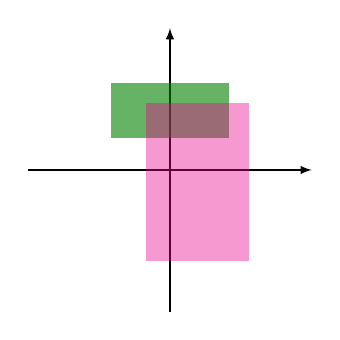
\begin{tikzpicture}[>=latex]
	% \draw [white] (-2,0) -- (-1.8,0);
	% \fill [red!20] (0,-1.8) rectangle (1.8,1.8);
	% \fill [blue!20] (0,-1.8) rectangle (-1.8,1.8);
	\draw [->] (-1.8,0) -- (1.8,0);
	\draw [->] (0,-1.8) -- (0,1.8);
	\fill [green!50!black , opacity=0.6] (-0.75,0.4) rectangle ++(1.5,0.7);
	\fill [magenta, opacity=0.4] (1,0.85) rectangle ++(-1.3,-2);
\end{tikzpicture}

\end{document}
